\documentclass[11pt]{article}
\usepackage[utf8]{inputenc}
\usepackage[a4paper, margin=2.5cm]{geometry}
\usepackage{tikz}
\usetikzlibrary{shapes,arrows.meta,fit}
\usetikzlibrary {positioning} %for relative positioning
\usepackage{graphicx}
\usepackage{xpatch} % for patching things in packages

\setlength{\parskip}{0cm}
\setlength{\parindent}{0cm}

\usepackage{fancyhdr}
 \setlength{\headheight}{39.49254pt}
\pagestyle{fancy}
\fancyhf{}
\lhead{Programmierpraktikum WiSe 2024/25\\Daszczynska, Oliwia Malgorzata (6950239)\\Kaiser, Sophie Renate Hildegard (6949963)}
\rhead{Bouaziz, Ishak (6774123)\\Vorontsov, Genadij (7697757)}

\author{Sophie Renate Hildegard Kaiser, Oliwia Malgorzata Daszczynska} % made it collaborating on Overleaf

\begin{document}
{\huge\textbf{Multimodal Parliament Explorer}}
\section*{1.c Project Planning and Design - Mock up Flowchart}

This Flowchart represents how the user will be able to navigate the webpages. It also explains what each site will display and how the user will be able to interact with the Parliament Explorer.
\\
\scalebox{0.9}{ % adjust size
\begin{tikzpicture}
\tikzset{
    state/.style={rectangle, draw, rounded corners, minimum width=3cm,minimum height=1cm,text width=4cm}
}

    % Navigation
    \node [state] (nav) {\vspace{-12px} \textbf{Navigation} \rule{\linewidth}{.5pt}
     • Home
    \\ •  Graphs
    \\ •  Speeches
    \\ •  Search
    \\ •  Export};

    % Graphs
    \node [state, below left=of nav] (graph) {\vspace{-12px} \textbf{Graphs} \rule{\linewidth}{.5pt}
    \\ • Bubble (Topic)
    \\ • Bar (POS)
    \\ • Radar (Sentiment)
    \\ • Sunburst (Named Entities)
    \rule{\linewidth}{.5pt}
    \textbf{Filters}:
    \\• all speeches
    \\• specific speech
    \\• specific set of speeches
    \\• by topic};

    % Speeches
    \node [state, right=2 of nav] (speeches) {
    \vspace{-12px} \textbf{Speech overview} \rule{\linewidth}{.5pt}
    list by session.\\
    filterable by speaker, topic, ...};
    \node [state, below=of speeches] (vs) {\vspace{-12px} \textbf{View a Speech} \rule{\linewidth}{.5pt}
    • Member picture, member info
    \\• Full text with comments.
    \\• Sentiment icons after each sentence
    \\• Toggle-able POS highlighting
    \\• Video Player with live highlighting};

    \node [state, left=2 of nav] (search) {\textbf{Search}}; 

    % Export
    \node [state, below=3of nav] (export) {\vspace{-12px} \textbf{Export} \rule{\linewidth}{.5pt}
    Options:
    \\• choose speech(es) (for speaker, topic, all speeches),
    \\• choose format (xmi, latex)};

    \draw [<->] (graph) -- (nav);
    \draw [<->] (search) -- (nav);
    \draw [<->] (export) -- (nav);
    \draw [<->] (speeches) -- (nav);
    \draw [->] (speeches)--(vs);

  
\end{tikzpicture}
}

\section*{1.c Project Planning and Design - Mock up user interface}
\subsection*{1.c.1 Home page}
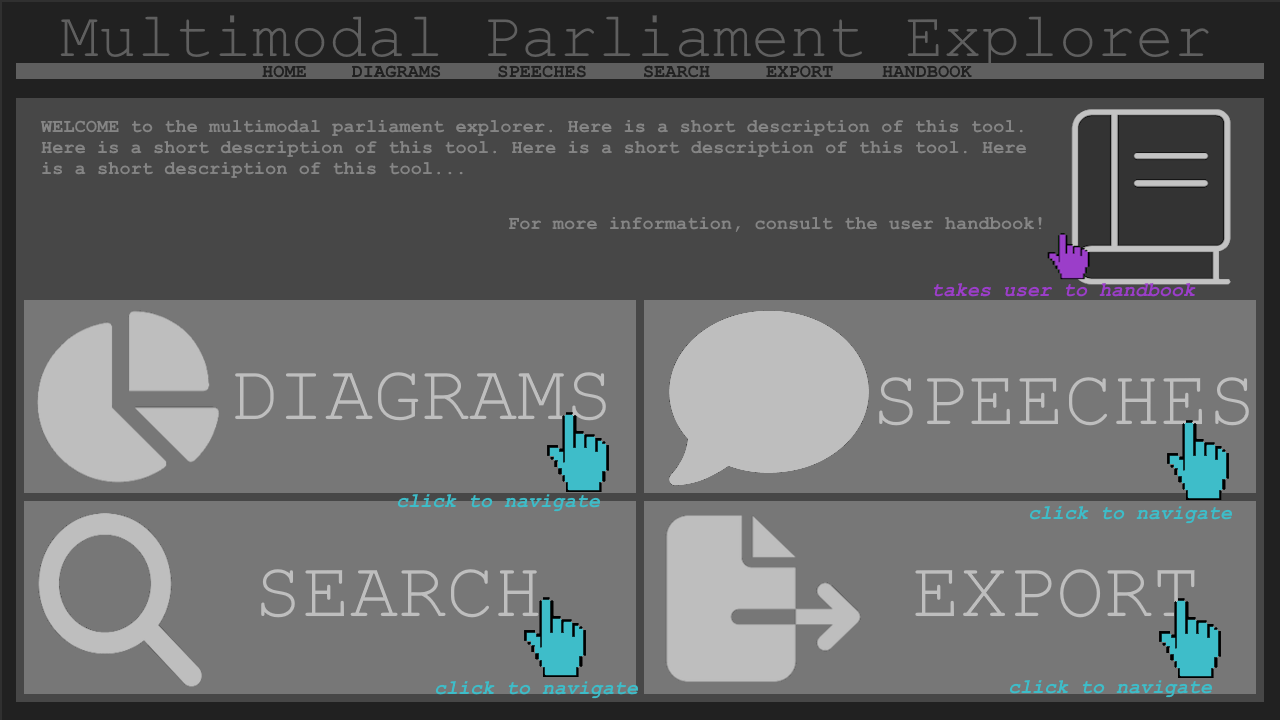
\includegraphics[scale=0.5]{home_page.png}
\subsection*{1.c.2 graph navigation and example}
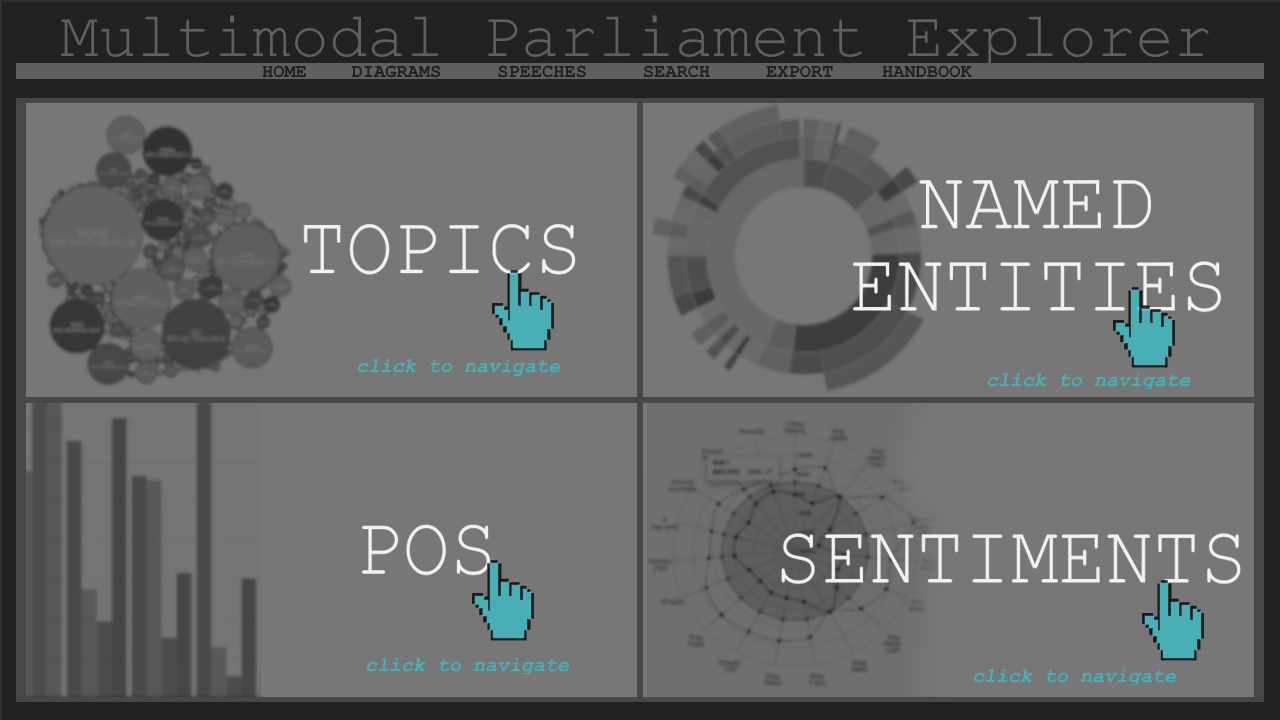
\includegraphics[scale=0.5]{graph_navigation.png}
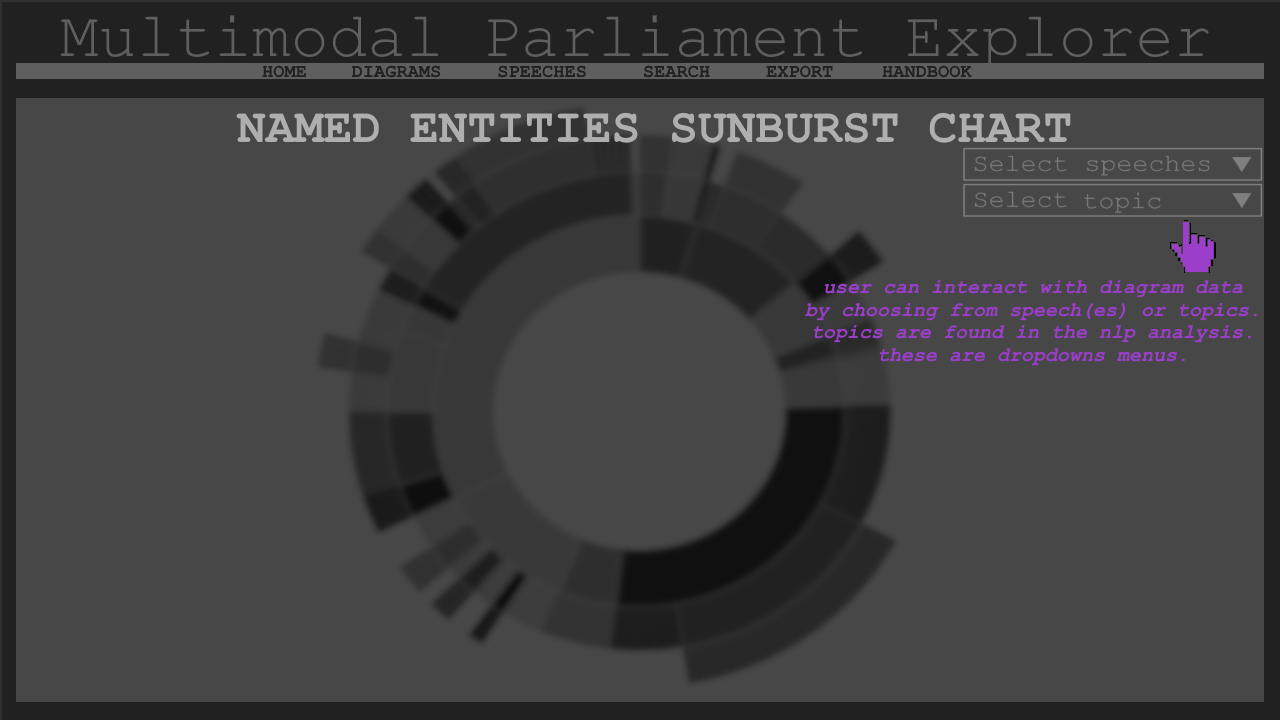
\includegraphics[scale=0.5]{graph_example.png}
\subsection*{1.c.3 Speech overview and page example}
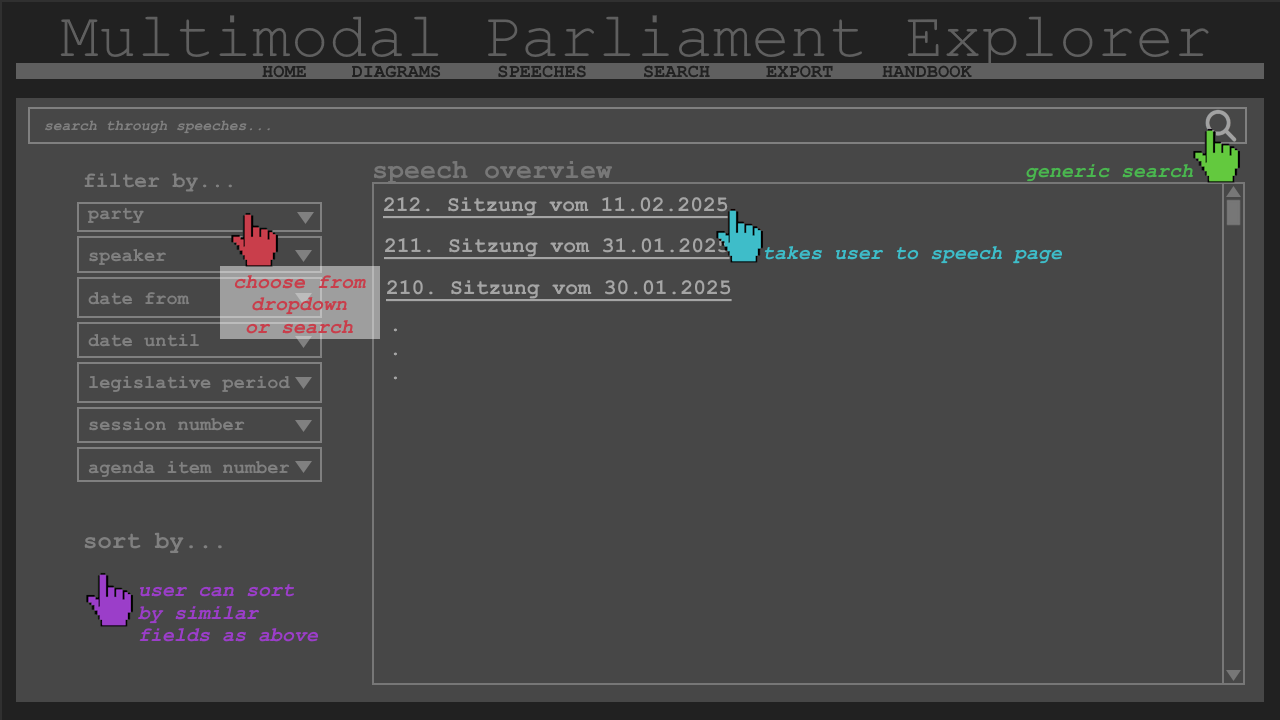
\includegraphics[scale=0.5]{speeches_overview.png}
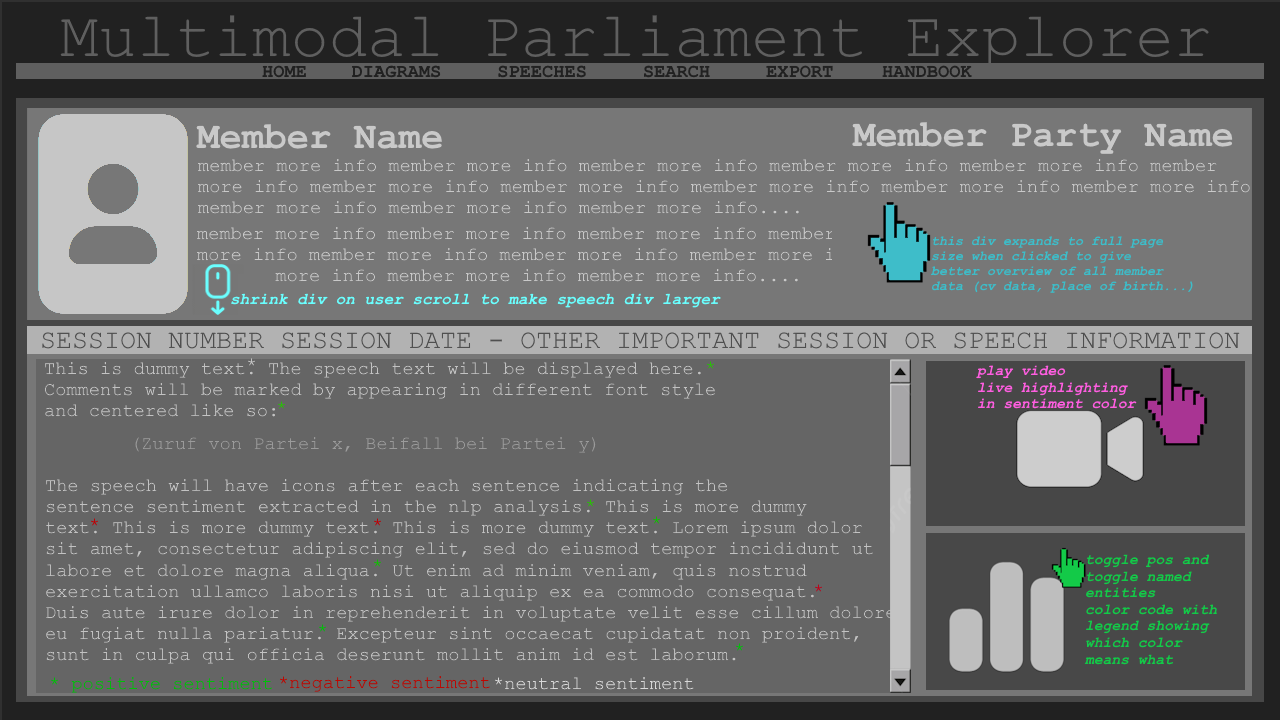
\includegraphics[scale=0.5]{speech_page_example.png}
\subsection*{1.c.4 export}
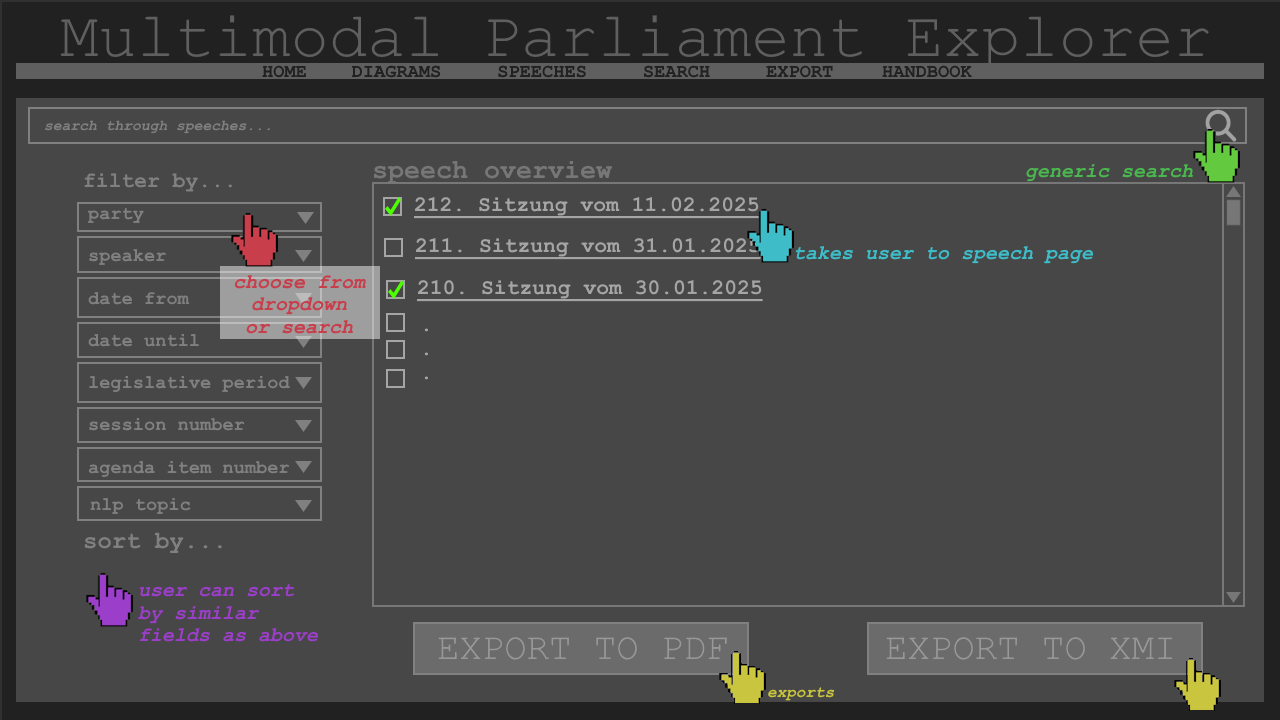
\includegraphics[scale=0.5]{export.png}
\end{document}